%!TEX root = main.tex

\section{Motivation}

\begin{frame}{Motivation}
    \begin{block}{Why do we care?}
      \begin{itemize}
          \item password cracking has an inherent parallel structure
          \item FPGAs enable to exploit true parallelism
      \end{itemize}
      \begin{itemize}
          \item bcrypt claims to resist hardware optimizations
          \item implementation presented last year\footnote{\tiny \url{http://www.openwall.com/presentations/Passwords13-Energy-Efficient-Cracking/}} (GSoC) can be optimized
      \end{itemize}
    \end{block}
\end{frame}
\note{\begin{itemize}
\item OpenWall bcrypt implementation on different platforms: \begin{itemize}
\item (mainly) parallela/epiphany board
\item zedboard
\item Xeon Phi
\item Haswell\end{itemize}
\item Problems with FPGA implementation: \begin{itemize}
\item only implemented cost loop in fabric
\item wait cycles
\item 14 cores with very unbalanced resource utilization\end{itemize}
\end{itemize}}

\section{bcrypt}

\begin{frame}{What is bcrypt?}
    Introduced in 1999 by Provos and Mazi\`{e}res.\footnote{\tiny \url{http://www.usenix.org/events/usenix99/full_papers/provos/provos.pdf}}
    \begin{columns}[T]
      \uncover<1->{
      \begin{column}{.45\textwidth}
        \begin{block}{bcrypt}
          \begin{itemize}
            \item cost-parameterized
            \item uses EksBlowfishSetup (key schedule) and encryption
          \end{itemize}
        \end{block}
      \end{column}}
      \uncover<2->{
      \begin{column}{.45\textwidth}
        \begin{block}{EksBlowfish}
          \begin{itemize}
            \item block cipher
            \item based on blowfish
            \item expensive key schedule
            \item encryption as in blowfish
          \end{itemize}
        \end{block}
      \end{column}}
    \end{columns}
    \vspace{5mm}
    Implemented in OpenBSD 2.1, Ruby on Rails, and PHP as standard password hash.
\end{frame}
\note{\begin{itemize}
\item proposed two constructions
\item \emph{bcrypt} cost parameterized hash function
\item cost factor controls computational effort of \texttt{EksBlowfishSetup}
\item \emph{EksBlowfish} less known, serves as underlying building block for bcrypt
\item itself is based on blowfish, expensive key schedule
\item practical applications in OpenBSD, Ruby on Rails, PHP
\item We start with explaining the key schedule
\end{itemize}}

\begin{frame}{EksBlowfish}
    \center
      \begin{block}{Pseudo code}
        \begin{algorithm2e}[H]
          \KwIn{cost, salt, key}
          \KwOut{state}
          $state \leftarrow$ InitState$()$\;
          $state \leftarrow$ ExpandKey$(state, salt, key)$\;
          \KwSty{Repeat} ($2^{cost}$) \Begin{
            $state \leftarrow$ ExpandKey$(state, 0, salt)$\;
            $state \leftarrow$ ExpandKey$(state, 0, key)$\;
          }
          \KwRet{$state$}\;
          \caption{EksBlowfishSetup}
        \end{algorithm2e}
      \end{block}
\end{frame}
\note{\begin{itemize}
\item state consists of 4 SBoxes, each 256 $\times$ \SI{32}{\bit} and
\item 18 \SI{32}{\bit} P-values (subkeys) $\Rightarrow$ \SI{4}{\kilo\byte} memory
\item initialized with digits of $\pi$
\item \texttt{ExpandKey} updates state (see next slide)
\item number of iterations exponential in cost parameter
\item $ExpandKey(state, 0, .)$ equals blowfish key schedule
\item encryption equals blowfish encryption
\end{itemize}}

\begin{frame}{ExpandKey}
    \center
    \begin{block}{ExpandKey(state, salt, key)}
      \begin{itemize}
          \item modified version of blowfish key schedule
          \item XORes key onto subkeys
          \item state update -- \emph{does not use key}
          \item 521 \texttt{bf\_enc} calls
      \end{itemize}
    \end{block}
    \begin{block}{State Update}
        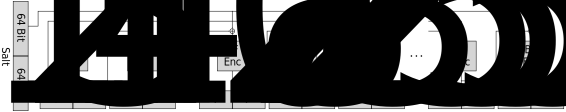
\includegraphics[width=\textwidth]{data/bcrypt_expandkey.pdf}
    \end{block}
\end{frame}
\note{\begin{itemize}
\item \texttt{ExpandKey} starts with xoring the key onto the subkeys
\item then blowfish encrypts lower \SI{64}{\bit} of Salt
\item Result substitutes $P_1$, $P_2$ and
\item gets xored with higher \SI{64}{\bit} of Salt, encrypted again\ldots
\item Altogether 521 blowfish encryptions per call
\item How does blowfish encryption works?
\end{itemize}}

%\begin{frame}{blowfish encryption}
%    \center \includegraphics[height=.80\textheight]{data/blowfish.pdf}
%\end{frame}
%\note{\begin{itemize}
%\item simple 16 round Feistel network
%\item in every round: key xor, f-Function xor, swap
%\item f-Function consists of 4 SBox look ups, 2 additions, 1 xor
%\item finalize: xor $P_{17}$, $P_{18}$
%\item \SI{64}{\bit} block size
%\item[$\Rightarrow$] nice minimalistic structure
%\end{itemize}}

\begin{frame}{bcrypt}
    \center
      \begin{block}{Pseudocode}
        \begin{algorithm2e}[H]
          \KwIn{cost, salt, key}
          \KwOut{hash}
          $state \leftarrow$ EksBlowfishSetup$(cost,salt,key)$\;
          $ctext \leftarrow$ ``OrpheanBeholderScryDoubt''\;
          \KwSty{Repeat} ($64$) \Begin{
            $ctext \leftarrow$ EncryptECB$(state, ctext)$\;
          }
          \KwRet{Concatenate$(cost,salt,ctext)$}\;
          \caption{bcrypt}
        \end{algorithm2e}
      \end{block}
\end{frame}
\note{\begin{itemize}
\item bcrypt itself is quite simple
\item calls \texttt{EksBlowfishSetup} followed by
\item 64 blowfish encryptions in ECB mode of  magic value (3 blocks)
\item[$\Rightarrow$] almost all work/time is spent during key schedule
\end{itemize}}

%\begin{frame}{Where are we?}
%    \begin{block}{bcrypt}
%    \begin{itemize}
%        \item based on blowfish
%        \item cost-parameterized password hash
%        \item inherent sequential structure
%        \item exponential (in \emph{cost}) loop iterations
%        \item \SI{4}{\kilo\byte} memory
%        \item randomly accessed
%    \end{itemize}
%    \end{block}
%\end{frame}
%\note{\begin{itemize}
%\item bcrypts cost depend only on many sequential blowfish encryption
%\item authors claim randomly accessed memory is costly
%\end{itemize}}

\section{Design of Implementation}
\begin{frame}{Design}
    \center \includegraphics[height=75mm]{data/cracker.png}
\end{frame}
\note{\begin{itemize}
\item we have no chance to parallelize bcrypts structure
\item does the memory consumption hurt?
\item depends on target FPGAs
\end{itemize}}

\begin{frame}{Target Platforms}{zedboard}
    Low cost, low power FPGA
    \begin{columns}[T]
      \begin{column}{.5\textwidth}
        \begin{block}{Specs}
          \begin{itemize}
            \item Zynq-7000 XC7Z020 FPGA (comparable to Artix7)
            \item ARM Cortex A9 CPU
            \item HDMI, VGA, Ethernet, Audio, USB, JTAG, SD Card, Buttons\ldots
            \item 140 \SI{36}{\kilo\bit} BRAMs
          \end{itemize}
        \end{block}
      \end{column}
      \begin{column}{.45\textwidth}
        \includegraphics[width=\textwidth]{data/zedboard.png}
      \end{column}
    \end{columns}
\end{frame}
\note{\begin{itemize}
\item OpenWall project also targeted zedboard
\item combines ARM Cortex A9 with programmable logic
\item embedded Linux can be run from SD card
\end{itemize}}

\begin{frame}{Target Platforms}{RIVYERA}
    High Performance FPGA cluster
    \begin{columns}[T]
      \begin{column}{.5\textwidth}
        \begin{block}{Specs}
          \begin{itemize}
            \item 64 Spartan-6 LX150\\(available with up to 128)
            \item i7 CPU
            \item 16 GB RAM
            \item 268 \SI{36}{\kilo\bit} BRAMs per FPGA
          \end{itemize}
        \end{block}
      \end{column}
      \begin{column}{.45\textwidth}
        \vspace{10mm}
        \includegraphics[width=\textwidth]{data/rivyera.png}
      \end{column}
    \end{columns}
    \vspace{5mm}
    Up to 10 RIVYERAs can be fit into a standard rack.
\end{frame}
\note{\begin{itemize}
\item \textsc{rivyera} is the actual FPGA cluster available @ EmSec
\item contains up to 128 Spartan6 (ours: 64)
\end{itemize}}

\begin{frame}{Optimization Goal}
    \center \Huge
    Low Area Footprint
\end{frame}
\note{
Design Goal?
\begin{itemize}
\item simple Feistel structure will allow high clock rates
\item[$\Rightarrow$] keep area footprint as low as possible
\item[$\Rightarrow$] fit as many cores onto on FPGA as possible
\end{itemize}}

\begin{frame}{Design}
    \begin{block}{API}
      \begin{itemize}
        \item keep API minimalistic $\Rightarrow$ low bandwidth interface
        \item transfer target \emph{salt} and \emph{hash}, start cracker
        \item on success, read \emph{password}
      \end{itemize}
    \end{block}
    \begin{block}{Password Generation}
      \begin{itemize}
        \item on-chip password generation
        \item no bandwidth
        \item split password range at synthesis-time
      \end{itemize}
      \begin{itemize}
        \item alternatively replace generator with interface for dictionary attacks
      \end{itemize}
    \end{block}
\end{frame}
\note{\begin{itemize}
\item minimalistic API results in low area consumption
\item password generation can be done efficiently in hardware
\end{itemize}}

\begin{frame}{Design}
    \begin{block}{bcrypt Core}
      \begin{itemize}
        \item memory for SBoxes, subkeys, key and initial values
        \item estimated almost no logic needed for algorithm\\consists mainly of BRAM access
      \end{itemize}
    \end{block}
    \begin{alertblock}{Problematic}
      \begin{itemize}
        \item memory for password storage\\registers require too much logic
        \item one core consumes more LUTs than expected\\need to optimize FSM, share resources
      \end{itemize}
    \end{alertblock}
\end{frame}
\note{\begin{itemize}
\item 2 SBoxes per BRAM, subkeys in 1 extra Bram
\item initial values take another 2 BRAMs (can be shared)
\item but: how to store passwords?
\item registers in logic are to costly
\item[$\Rightarrow$] quad-core design
\end{itemize}}

\begin{frame}{Design}
    \begin{block}{Quad Core}
      \begin{itemize}
        \item bundle four bcrypt cores together
        \item store four passwords in one BRAM
        \item during initialization, password generator can access BRAM
        \item core0, core1 and core2, core3 access the BRAM alternately
      \end{itemize}
    \end{block}
    \begin{exampleblock}{Advantages}
      \begin{itemize}
        \item cores need access only during begin of \texttt{ExpandKey}\\thus,
              they only diverge by 36 clock cycles
        \item saves more than 4000 LUTs per quad core\\
              \SI{20}{\percent} per single core
      \end{itemize}
    \end{exampleblock}
\end{frame}
\note{\begin{itemize}
\item dual port BRAM allows 2 read/write accesses per clock
\item bundle 4 cores, alternate their memory access phases
\item password generator can access the memory during 256 initialization cycles
\item cores diverge only by 36 clock cycles
\end{itemize}}

\begin{frame}{Resulting Design}
    \begin{block}{Quad Core}
    \center 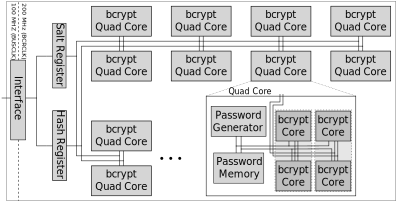
\includegraphics[width=.90\textwidth]{data/bcrypt_design_overview.pdf}
    \end{block}
\end{frame}
\note{\begin{itemize}
\item every quad core operates fully independent on his own password subrange
\end{itemize}}

\begin{frame}{Resulting Design}
    \begin{block}{Password Generation}
    \center 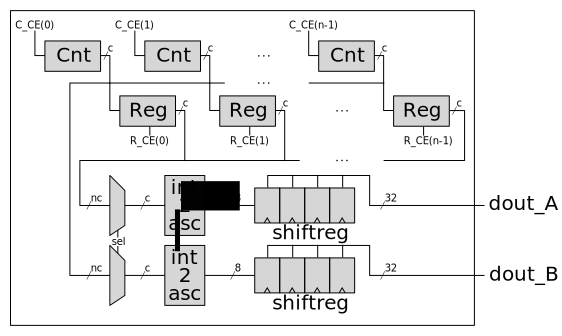
\includegraphics[width=.90\textwidth]{data/password_gen.pdf}
    \end{block}
\end{frame}
\note{\begin{itemize}
\item simple structure
\item low resource requirements
\item control logic:\begin{itemize}
\item update counter once
\item save state in register
\item update counter again
\item map counter / register state according to \textsc{int2asc} to \textsc{ascii}
\item load shiftreg and write \SI{32}{\bit} words to BRAM\end{itemize}
\end{itemize}}

% \begin{frame}{How to interface the FPGA}
%     Different possibilities for zedboard:
%     \begin{itemize}
%         \item AXI4 Interfaces \begin{itemize}
%             \item[+] low area footprint
%             \item[--] more complex to implement
%             \end{itemize}
%         \item Xillybus \begin{itemize}
%             \item[+] abstracts from AXI4 Interfaces
%             \item[+] Linux support $\Rightarrow$ easy to demonstrate
%             \item[--] proprietary
%             \item[--] \enquote{fat}, i.e.\, higher resource consumption
%             \end{itemize}
%     \end{itemize}
%     Custom interface for \textsc{rivyera} needed.
% \end{frame}
% \note{\begin{itemize}
% \item Linux driver allows DMA into logic
% \item host side interface consists only of file write/reads.
% \item Status Register:\begin{itemize}
% \item low nibble used for host-to-FPGA communication (reset, start)
% \item high nibble used for FPGA-to-host communication (done, success)\end{itemize}
% \end{itemize}}

\begin{frame}{Resulting Resources}
    \begin{block}{zedboard}
      \begin{itemize}
          \item estimations for one zedboard:
          \item[] 28 cores as upper bound, BRAMs as limiting resource
          \item first design attempt (password in registers):
          \item[] 12 cores fit, LUT utilization way to high
          \item Quad Core Design:
          \item[] 24 cores fit, while using \enquote{big} interface
      \end{itemize}
    \end{block}
    \begin{block}{\textsc{rivyera}}
      \begin{itemize}
          \item Quad Core Design:
          \item[] 48 cores per Spartan-6 LX150 $\Rightarrow$ 3072 cores on whole \textsc{rivyera}
      \end{itemize}
    \end{block}
\end{frame}
\note{\begin{itemize}
\item with Xillybus 24 cores @ \SI{200}{\mega\hertz} possible (zedboard)
\item with custom interface 48 cores @ \SI{100}{\mega\hertz} possible (\textsc{rivyera})
\end{itemize}}

\section{Demo}
\begin{frame}{Demo}
    \center \includegraphics[height=50mm]{data/demo.png}
\end{frame}
\note{\begin{itemize}
\item demonstrate interface :-)
\end{itemize}}

\section{Results}
\begin{frame}{Results}
\begin{block}{Compared to OpenWall}
\begin{itemize}
  \item OpenWall (GSoC) 780 H/s (cost 5) -- zedboard 3,200 H/s
\end{itemize}
\end{block}
\vspace{-1mm}
\visible<2->{
\begin{block}{cost Parameter for Target (CPU) runtime}
\begin{table}[tp]
  \centering
  \begin{tabular}{l r r r r}
    \toprule
                & \SI{1}{\milli\second} & \SI{10}{\milli\second} & \SI{100}{\milli\second} & \SI{1000}{\milli\second} \\
    \midrule
    bcrypt cost & 3.69     & 7.03       & 10.3      & 13.6     \\
    \midrule
    i5-2400     & 1015 H/s & 101.88 H/s & 11.16 H/s & 1.15 H/s \\
    \bottomrule
  \end{tabular}
\end{table}
\end{block}
\vspace{-1.5mm}
resembles performance of server-side implementation\footnote{\tiny \url{http://www.openwall.com/crypt/}}}
\end{frame}
\note{\begin{itemize}
\item measured bcrypt runtime on different CPUs
\item[$\Rightarrow$] averaged cost factor
\item Hash-rates compared too previous cost factors
\item GPU Hash-rate measured with oclHashcat
\item[$\Rightarrow$] about 3 times faster than GTX 480
\end{itemize}}

\begin{frame}{Results}{Compared to CPUs and GPUs}
\begin{block}{Hash-rates }
\begin{table}[tp]
  \centering
  \begin{tabular}{l r r r r}
    \toprule
                        & \multicolumn{4}{c}{\small Hashs per Second}\\
    Target CPU runtime  & \SI{1}{\milli\second} & \SI{10}{\milli\second} & \SI{100}{\milli\second} & \SI{1000}{\milli\second} \\
    \midrule
    {\bf zedboard} & {\bf 9,230} & {\bf 916.25} & {\bf 98.77} & {\bf 9.93} \\
    Spartan-6 LX150& {9,230}     & {916.25}     & {98.77}     & {9.93}     \\
    Virtex-6 LX240T& 55,380      & 5,497.5      & 592.62      & 59.58      \\
    RIVYERA        & 590,720     & 58,640.0     & 6,321.28    & 635.52     \\
    \midrule
    i7-3820\,QM    &   4,800 &  477.71 &  51.0 &  4.6      \\
    Xeon E3-1240   &  14,738 & 1497.0 & 172.7 & 16.8      \\
    \midrule
    GTX 480    &  2,868 & 319.4 & 33.7 & 2.7 \\
    GTX 750 Ti &  4,794 & 478.8 & 52.7 & 4.6 \\
    \bottomrule
  \end{tabular}
\end{table}
\end{block}
\end{frame}

\begin{frame}{Results}{Besides pure Hash-rate}
    \begin{block}{zedboard}
      \begin{itemize}
        \item costs \$300--\$400 --- cheaper Zynq-7000 also boards available
        \item consumes up to \SI{5}{\watt}
        \item no overhead, everything is includes on board
      \end{itemize}
    \end{block}
\begin{columns}[T]
  \begin{column}{.45\textwidth}
    \begin{block}{GTX 480}
      \begin{itemize}
        \item \$500 in 2010
        \item \SI{430}{\watt}
      \end{itemize}
    \end{block}
  \end{column}
  \begin{column}{.45\textwidth}
    \begin{block}{GTX 750 Ti}
      \begin{itemize}
        \item \$150
        \item \SI{60}{\watt}
      \end{itemize}
    \end{block}
  \end{column}
\end{columns}
\end{frame}
\note{}

\begin{frame}{Optimizations}
    \begin{block}{To be done}
      \begin{itemize}
          \item \SI{200}{\mega\hertz} on zedboard, but only \SI{100}{\mega\hertz} on \textsc{rivyera}
          \item low FF/LUT ratio
          \item unused FFs can be used to buffer signals
          \item[] $\Rightarrow$ shorter critical path
          \item[] $\Rightarrow$ higher clock speed
          \item optimize the interface $\Rightarrow$ 28 cores per zedboard
      \end{itemize}
    \end{block}
\end{frame}
\note{}